\subsection{Physical plausibility on a coffee table}
We tested a simple interaction on the coffee table recovered by Inventory
from a held-out CA-1M living room (Figure~\ref{fig:physics}). The simulation
kept the table fixed and treated the five plates and tissue-box assembly
as dynamic bodies. We let the objects settle and then applied a
3\,N pulse for 0.0625\,s to the top plate. We measured motion relative to its
position just before the push.

All three density models passed the rest test. After two seconds of settling,
each object stayed within 2\,mm and $2^\circ$ of its reference pose, ended with
speed below 1\,mm/s over the final second and retained bounding-box contact
with its assigned support. The top plate moved 14.1\,mm under uniform density,
14.7\,mm under VoMP's average density and 14.7\,mm under its spatial density.
Changing friction had a larger effect in this scene. With spatial density
fixed, halving friction increased displacement to 44.6\,mm, while raising
friction by half reduced displacement to nearly zero.

\begin{figure}[!htbp]
\centering
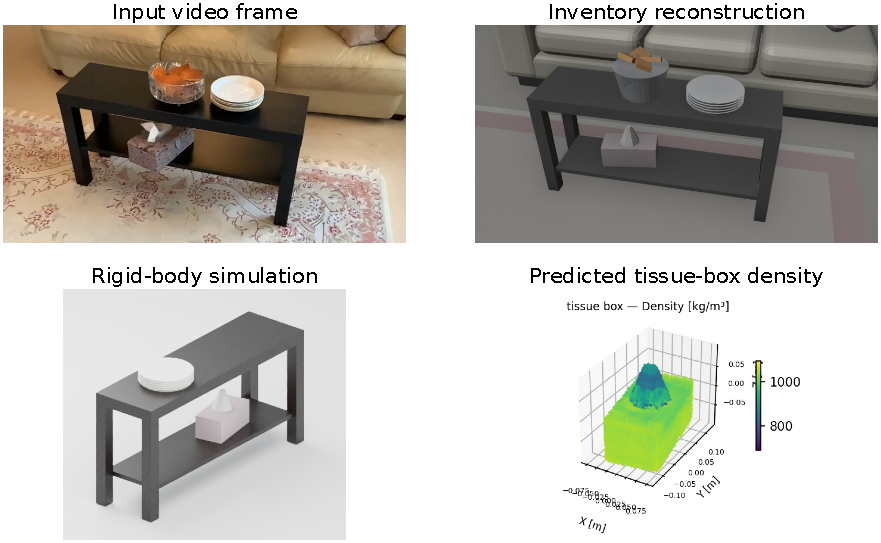
\includegraphics[width=0.93\linewidth]{figures/ca1m-coffee-physics.pdf}
\caption{From video to a physical test. The matched camera views (top) show
the plates on the tabletop and the tissue box on the shelf below. The simulation
uses those recovered meshes (bottom left). The predicted density field
(bottom right, kg/m$^3$) fills the solid tissue-box mesh, contributing to its
high estimated mass.}
\label{fig:physics}
\end{figure}

The tissue box passed the rest test, yet its estimated mass was 3.13\,kg.
Agent review flagged the mismatch between this estimate and the object's
hollow construction. The mesh occupied the equivalent of 3.08 liters of solid
material at near-water density. This explains how a stable simulation can
inherit a physically implausible mass. We lack measured masses and trajectories
for these objects, so the pilot establishes sensitivity to modeling choices.
